\documentclass[12pt]{article}

% Popup for cipher
\usepackage{pdfcomment}
% Draw Caesar cipher / LFSR
\usepackage{tikz}
\usetikzlibrary{matrix,positioning,calc,fit}
\tikzset{circ/.style={draw,circle,node distance=2mm,inner sep=0.1pt},topath/.style={to path={|-(\tikztotarget)}}}

\usepackage{ifthen}
% Be able to get substrings
\usepackage{xstring}

% Caesar cipher drawing
\newcounter{index}
%command to increase a counter by 1 modulo 26
\newcommand{\increase}[1]{\ifthenelse{\arabic{#1}<26}{\addtocounter{#1}{1}}{\setcounter{#1}{1}}}
\newcommand{\pOneCipher}{CBDGFAIELKHJMSNQOPURVTYWXZ}
\newcommand{\pOneKey}{ETANORSICLHDUPMGWFVYKBXJQZ}

% Standard
\usepackage[top=0.8in,bottom=0.8in]{geometry}
\usepackage{amsmath,bm}
\usepackage{amssymb}
\usepackage{enumitem}
\usepackage{graphicx}
\usepackage{tcolorbox}
\usepackage{array,multirow}
\usepackage{mathtools}
\DeclarePairedDelimiter{\ceil}{\lceil}{\rceil}
\DeclarePairedDelimiter\floor{\lfloor}{\rfloor}
% Enables font change size in verbatim blocks
\makeatletter
\newcommand{\verbatimfont}[1]{\renewcommand{\verbatim@font}{\ttfamily#1}}
\makeatother
\usepackage{hyperref}
\hypersetup{
    colorlinks=true,
    linkcolor=blue,
    filecolor=magenta,      
    urlcolor=cyan,
}
 
\urlstyle{same}


% Format for answering questions
\newenvironment{answer}
{ \begin{tcolorbox}[halign=left]
    }
    {  
  \end{tcolorbox}
}
   
\begin{document}

\title{CS 4801: Assignment 1}
\author{Adam Camilli (aocamilli@wpi.edu)}
\date{\today}
\maketitle

\begin{enumerate}
\item The ciphertext was encrypted using a substitution cipher. The
  objective is to decrypt the ciphertext without knowledge of the key.
  \begin{enumerate}
  \item Provide the relative frequency of all letters [A-Z] in the ciphertext \hspace{4cm}\pdfcomment[icon=Key, hspace=5cm,color=black]
  {CKCLBAELDK DGJ LFNSMBCA CGQEGCCAI JCUCKFS DGJ LACDBC SAFJMLBI BHDB LHDGQC
    BHC OFAKJ DGJ NDVC FMA KEUCI CDIECA BHC LCKK SHFGCI OC JCSCGJ FG BHC LFNSMBCAI
    MICJ EG GDBEFGDK ICLMAEBR DGJ BHC CKCLBAELDK IRIBCNI BHDB NDVC FMA LDAI
    FSCADBC OCAC DKK LACDBCJ TR CKCLBAELDK DGJ LFNSMBCA CGQEGCCAI DB OSE OC
    VCCS BHDB SAFQACII NFUEGQ PFAODAJ OEBH FMA EGGFUDBEUC ACICDALH DGJ FMB-FP-
    BHC TFY DSSAFDLHCI BHC JCSDABNCGB FP CKCLBAELDK DGJ LFNSMBCA
    CGQEGCCAEGQ DB OSE LHDKKCGQCI IBMJCGBI BF SMIH BHCNICKUCI BF MGJCAIBDGJ
    IFLECBRI DGJ BCLHGFKFQRI LFNSKCY EIIMCI EG D TAFDJCA LFGBCYB BHDG OHDBI EG
    PAFGB FP BHCN OC ODGB FMA IBMJCGBI OHCBHCA BHCR DAC CDAGEGQ DG
    MGJCAQADJMDBC NEGFA FA D JFLBFADBC BF BDLVKC IFLECBRI NFIB SACIIEGQ SAFTKCNI
    DGJ MGLFUCA GCO ODRI FP IFKUEGQ BHCN OHCBHCA EBI JCUCKFSEGQ IRIBCNI BHDB LDG
    KFLDBC PEACPEQHBCAI EG BHC NEJJKC FP D TMAGEGQ TMEKJEGQ FA LACDBEGQ
    GCMAFSAFIBHCBELI BHDB KFFV DGJ PMGLBEFG KEVC GDBMADK KENTI FMA PDLMKBR DGJ
    IBMJCGBI DAC DB BHC PAFGB CJQC FP ACNDAVDTKC EGGFUDBEFG OHEKC DJUDGLEGQ
    BCLHGFKFQECI EI DB FMA LFAC OC DKIF BDVC HMNDG LFGGCLBEFGI UCAR ICAEFMIKR EG
    CLC OC SAEJC FMAICKUCI FG BHC PDNEKR-KEVC DBNFISHCAC OC LMKBEUDBC; PDLMKBR
    IBMJCGBI DGJ IBDPP CGLFMADQC CDLH FBHCAI CUCAR IMLLCII DGJ DAC BHCAC PFA BHC
    LHDKKCGQCI TFBH EG BHC LKDIIAFFN DGJ EG KEPC}
  \begin{answer}
    \begin{center}
      \begin{tabular}{c|c|c}
        \textbf{Letter} & \textbf{Appearances} & \textbf{Relative Frequency} \\
        \hline
        C & 150 & 13.93\% \\
        \hline
        B & 100 & 9.29\% \\
        \hline
        D & 86 & 7.99\% \\
        \hline
        G & 83 & 7.71\% \\
        \hline
        F & 76 & 7.06\% \\
        \hline
        A & 75 & 6.96\% \\
        \hline
        I & 70 & 6.5\% \\
        \hline
        E & 58 & 5.39\% \\
        \hline
        L & 50 & 4.64\% \\
        \hline
        K & 47 & 4.36\% \\
        \hline
        H & 45 & 4.18\% \\
        \hline
        J & 40 & 3.71\% \\
        \hline
        M & 37 & 3.44\% \\
        \hline
        S & 24 & 2.23\% \\
        \hline
        N & 24 & 2.23\% \\
        \hline
        Q & 23 & 2.14\% \\
        \hline
        O & 19 & 1.76\% \\
        \hline
        P & 19 & 1.76\% \\
        \hline
        U & 15 & 1.39\% \\
        \hline
        R & 15 & 1.39\% \\
        \hline
        V & 9 & 0.84\% \\
        \hline
        T & 9 & 0.84\% \\
        \hline
        Y & 3 & 0.28\% \\
        \hline
        W & 0 & 0.0\% \\
        \hline
        X & 0 & 0.0\% \\
        \hline
        Z & 0 & 0.0\% \\
      \end{tabular}
    \end{center}
  \end{answer}
    \newpage
    
  \item Decrypt the ciphertext with help of the relative letter frequency of the English language (e.g., search Wikipedia for letter frequency analysis). Note that the text is relatively short and might not completely fulfill the given frequencies from the table.
    \begin{answer}
      By comparing the letter frequencies in the above table to those of the English language, and then some of the most common bigrams and trigrams within the text to common English words such as ``THE'', ``BE'', ``AND'', ``IN'', etc., I was able to decrypt the ciphertext: \pdfcomment[icon=Key,color=yellow]
      {ELECTRICAL AND COMPUTER ENGINEERS DEVELOP AND CREATE PRODUCTS THAT CHANGE THE WORLD AND MAKE OUR LIVES EASIER THE CELL PHONES WE DEPEND ON THE COMPUTERS USED IN NATIONAL SECURITY AND THE ELECTRICAL SYSTEMS THAT MAKE OUR CARS OPERATE WERE ALL CREATED BY ELECTRICAL AND COMPUTER ENGINEERS AT WPI WE KEEP THAT PROGRESS MOVING FORWARD WITH OUR INNOVATIVE RESEARCH AND OUT-OF-THE BOX APPROACHES THE DEPARTMENT OF ELECTRICAL AND COMPUTER ENGINEERING AT WPI CHALLENGES STUDENTS TO PUSH THEMSELVES TO UNDERSTAND SOCIETYS AND TECHNOLOGYS COMPLEX ISSUES IN A BROADER CONTEXT THAN WHATS IN FRONT OF THEM WE WANT OUR STUDENTS WHETHER THEY ARE EARNING AN UNDERGRADUATE MINOR OR A DOCTORATE TO TACKLE SOCIETYS MOST PRESSING PROBLEMS AND UNCOVER NEW WAYS OF SOLVING THEM WHETHER ITS DEVELOPING SYSTEMS THAT CAN LOCATE FIREFIGHTERS IN THE MIDDLE OF A BURNING BUILDING OR CREATING NEUROPROSTHETICS THAT LOOK AND FUNCTION LIKE NATURAL LIMBS OUR FACULTY AND STUDENTS ARE AT THE FRONT EDGE OF REMARKABLE INNOVATION WHILE ADVANCING TECHNOLOGIES IS AT OUR CORE WE ALSO TAKE HUMAN CONNECTIONS VERY SERIOUSLY IN ECE WE PRIDE OURSELVES ON THE FAMILY-LIKE ATMOSPHERE WE CULTIVATE; FACULTY STUDENTS AND STAFF ENCOURAGE EACH OTHERS EVERY SUCCESS AND ARE THERE FOR THE CHALLENGES BOTH IN THE CLASSROOM AND IN LIFE}:
      \newline
    \end{answer}    
  \item Find the key and provide letter frequency for the given text.
    \begin{answer}
      The letter frequency of the resulting plaintext is:
      \begin{center}
        \begin{tabular}{c|c|c}
          \textbf{Letter} & \textbf{Appearances} & \textbf{Relative Frequency} \\
          \hline
          E & 150 & 13.93\% \\
          \hline
          T & 100 & 9.29\% \\
          \hline
          A & 86 & 7.99\% \\
          \hline
          N & 83 & 7.71\% \\
          \hline
          O & 76 & 7.06\% \\
          \hline
          R & 75 & 6.96\% \\
          \hline
          S & 70 & 6.5\% \\
          \hline
          I & 58 & 5.39\% \\
          \hline
          C & 50 & 4.64\% \\
          \hline
          L & 47 & 4.36\% \\
          \hline
          H & 45 & 4.18\% \\
          \hline
          D & 40 & 3.71\% \\
          \hline
          U & 37 & 3.44\% \\
          \hline
          P & 24 & 2.23\% \\
          \hline
          M & 24 & 2.23\% \\
          \hline
          G & 23 & 2.14\% \\
          \hline
          W & 19 & 1.76\% \\
          \hline
          F & 19 & 1.76\% \\
          \hline
          V & 15 & 1.39\% \\
          \hline
          Y & 15 & 1.39\% \\
          \hline
          K & 9 & 0.84\% \\
          \hline
          B & 9 & 0.84\% \\
          \hline
          X & 3 & 0.28\% \\
          \hline
          J & 0 & 0.0\% \\
          \hline
          Q & 0 & 0.0\% \\
          \hline
          Z & 0 & 0.0\% \\
        \end{tabular}
      \end{center}
    \end{answer}
  \newpage
  \begin{answer}
    and the key is:
    \begin{center}
      \setcounter{index}{26}
      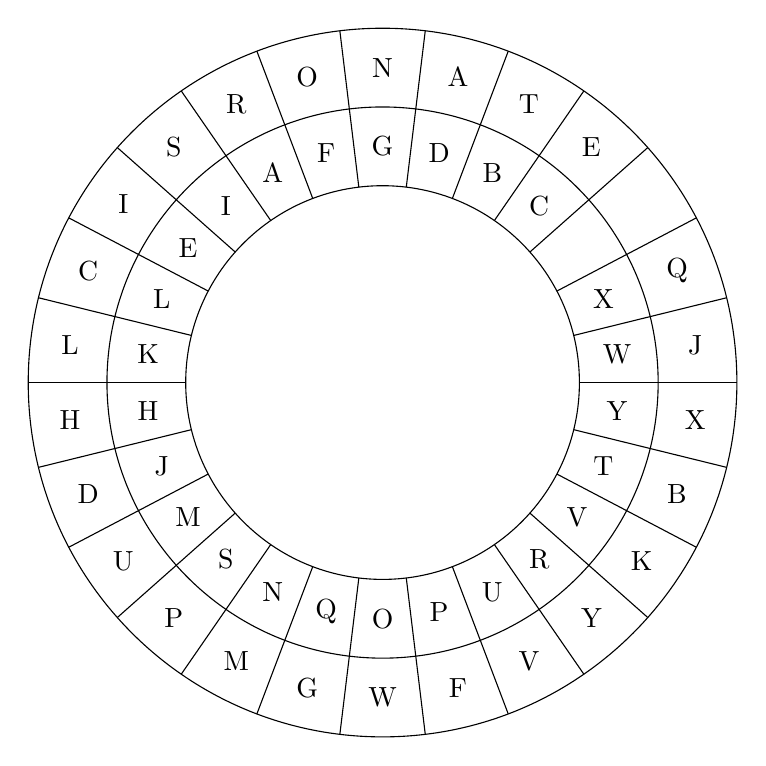
\begin{tikzpicture}[scale=0.5]
        \draw(0,0)circle(5)circle(7)circle(9);
        \foreach \x in {1,2,...,26}
        {
          \draw(\x*360/26:5)--(\x*360/26:9);
          \node at (\x*360/26+360/26+180/26:6){\StrMid{\pOneCipher}{\arabic{index}}{\arabic{index}}};
          \node at (\x*360/26+360/26+180/26:8){\StrMid{\pOneKey}{\arabic{index}}{\arabic{index}}};
          \increase{index}
        }
      \end{tikzpicture}
    \end{center}
  \end{answer}

  \end{enumerate}

\item Modular arithmetic is the basis of many cryptosystems. As a consequence, we will address this topic with several problems in this and upcoming chapters.
  \begin{enumerate}
  \item Compute the results:
    \begin{enumerate}
    \item $27 \cdot 13 \bmod 23$
      \begin{answer}
        {\begin{align*}
           27 \cdot 13 & \equiv 351 \bmod 23 & \\
                                & = \bm{6} & \left(351 - 23 \cdot \floor*{\frac{351}{23}} = 6 \right) \\
         \end{align*}}
     \end{answer}
   \item $17 \cdot 13 \bmod 23$
     \begin{answer}
       {\begin{align*}
          17 \cdot 13 & \equiv 221 \bmod 23 & \\
                      & = \bm{14} & \left(221 - 23 \cdot \floor*{\frac{221}{23}} = 14 \right)\\
        \end{align*}}
    \end{answer}
    \newpage
  \item $28 \cdot 15 \bmod 12$
    \begin{answer}
      {\begin{align*}
           28 \cdot 15 & \equiv 420 \bmod 12 & \\
                                & = \bm{0} & \left(12\cdot 35 = 420 \right)\\
         \end{align*}}
     \end{answer}
   \item $15 \cdot 29 + 11 \cdot 15 \bmod 23$
     \begin{answer}
        {\begin{align*}
           15 \cdot 29  &+ 11 \cdot 15 \bmod 23 & \\
                        &= 40 \cdot 15 \bmod 23 & \\
                        & \equiv 600 \bmod 23 & \\
                        & = \bm{2} & \left(600 - 26 \cdot \floor*{\frac{600}{23}} = 2 \right)\\
         \end{align*}}
     \end{answer}
   \end{enumerate}
   
  \item Find the inverses in the given modular spaces:
    \begin{enumerate}
    \item $4^{-1} \bmod 17$
      \begin{answer}
        \begin{align*}
          &\texttt{gcd(}4,17\texttt{)} = 1 & \text{(Solution exists)} \\
          &4 \bmod 17 = 4 & (17 \cdot 0 + 4 = 4)\\
          &4 \cdot 0 \equiv 0 \text{ } \bmod 17 & \\
          &\ldots & \text{(Run Euclid's algorithm)} \\
          &4 \cdot 13 \equiv 68 \text{ } (\bmod \text{ } 17) \equiv 1 \text{ } (\bmod \text{ } 17)  & \\
          &4 \cdot 13 = 1 + 17 \cdot 3 & \text{Modular inverse is \textbf{13}} \\
        \end{align*}
      \end{answer}
    \item $5^{-1} \bmod 37$
      \begin{answer}
        \begin{align*}
          &\texttt{gcd(}5,37\texttt{)} = 1 & \text{(Solution exists)} \\
          &5 \bmod 37 = 5 & (37 \cdot 0 + 5 = 5)\\
          &5 \cdot 0 \equiv 0 \text{ } \bmod 37 & \\
          &\ldots & \text{(Run Euclid's algorithm)} \\
          &5 \cdot 15 \equiv 75 \text{ } (\bmod \text{ } 37) \equiv 1 \text{ } (\bmod \text{ } 37)  & \\
          &5 \cdot 15 = 1 + 37 \cdot 2 & \text{Modular inverse is \textbf{15}} \\
        \end{align*}
      \end{answer}
    \item $7^{-1} \bmod 17$
      \begin{answer}
        \begin{align*}
          &\texttt{gcd(}7,17\texttt{)} = 1 & \text{(Solution exists)} \\
          &7 \bmod 17 = 7 & (17 \cdot 0 + 7 = 7)\\
          &7 \cdot 0 \equiv 0 \text{ } \bmod 17 & \\
          &\ldots & \text{(Run Euclid's algorithm)} \\
          &7 \cdot 5 \equiv 35 \text{ } (\bmod \text{ } 17) \equiv 1 \text{ } (\bmod \text{ }17)  & \\
          &7 \cdot 5 = 1 + 17 \cdot 2 & \text{Modular inverse is \textbf{5}} \\
        \end{align*}
      \end{answer}
    \item $10^{-1} \bmod 15$
       \begin{answer}
        \begin{align*}
          &\texttt{gcd(}10,15\texttt{)} = 5 & \textbf{(Solution does not exist)} \\
        \end{align*}
      \end{answer}
    \end{enumerate}
    
  \end{enumerate}

  \newpage
  
\item List all elements of modulo 36 with no multiplicative inverse.
  \begin{answer}
    The elements of a modulo $n$ are defined as
    \[ \bmod \text{ }n \equiv \mathbb{Z}_n = \{0, 1,\ldots, n-1 \}\]
    By the existence property of the modular multiplicative inverse,
    \[ \exists \text{ } a^{-1} \mid aa^{-1} \equiv 1 \text{ }(\bmod\text{ } n) \Longleftrightarrow a \perp n\]
    i.e. an element $a$ of modulo $n$ will have a multiplicative inverse $\bmod\text{ } n$ if and only if it is coprime to $n$.
    \\~\\ Since zero has no real reciprocals, it and any element of $\mathbb{Z}_{36}$ which shares a non-trivial factor with 36 should be listed. We can take the prime factorization of 36
    \[ 36 = 2^2 \cdot 3^2 \]
    and simply list all elements of $\mathbb{Z}_{36}$ which share one of these factors:
    \begin{align*}
      \{\} &: \{0\} \\
      \{2\} &: \{2, 4, 6, 8, 10, 12, 14, 16, 18, 20, 22, 24, 26, 28, 30, 32, 34\}\\
      \{3\} &: \{3, 6, 9, 12, 15, 18, 21, 24, 27, 30, 33\}\\     
    \end{align*}
    \[\bm{\{0, 2, 4, 6, 8, 9, 10, 12, 14, 15, 16, 18,}\]
    \[\text{\hspace{1cm}}\bm{20, 21, 22, 24, 26, 27, 28, 30, 32, 33, 34\}}\]
  \end{answer}

\item An LFSR is given by
  \[ (9, (C_0 , C_1 , \ldots, C_8), (Z_0 , Z_1, \ldots, Z_8)) = (9, x^8 + x^6 + x^5 + x^4 + 1, (0,0,0,1,1,0,1,0,0)).* \]
  \begin{enumerate}
  \item Draw a circuit diagram for the given LFSR.
    \begin{answer}
      \begin{center}
        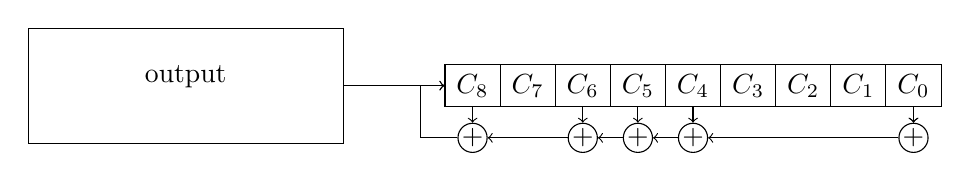
\begin{tikzpicture}
          % The LFSR chain + outputs
          \matrix (M) [matrix of math nodes,nodes={draw,minimum width=7mm},column sep=-\pgflinewidth,row sep=0.5cm]
          {
            C_{8} & C_7 & C_6 & C_5 & C_4 & C_3 & C_2 & C_1 & C_0 \\
          };

          % taps 
          \foreach \i/\j in {1/9, 1/5, 1/4, 1/3, 1/1}
          {\node (c-\i-\j) [circ,below=of M-\i-\j]{$+$};
            \draw[->] (M-\i-\j)--(c-\i-\j);}

          % arrows
          \draw[->] (M-1-9) edge (c-1-9) (c-1-9) edge (c-1-5) (c-1-5) edge (c-1-4) (c-1-4) edge (c-1-3) (c-1-3) edge (c-1-1) (c-1-1) -| ($(M-1-1.west)+ (-3mm,0)$)--(M-1-1);

          % output box
          \coordinate (flc1) at ($(M-1-1.south east) + (-2,1)$);
          \coordinate (frc1) at ($(M-1-1.north east) + (-6,-1)$);
          \node(s)[draw, fit=(flc1) (frc1),inner sep=0pt] {output};  
          \draw[->] (M-1-1 -| flc1)--(M-1-1);
          
        \end{tikzpicture}
      \end{center}
    \end{answer}
    \newpage
  \item Compute first 30 bits of the output bit stream
    \begin{answer}
      The output bit at each run can be simplified: Since XOR-gates are the function in use for this LFSR, one can determine the output of a given input by counting the odd bits that have on gates. An odd number means an output of 1, and an even number an output of 0.
      \begin{center}
        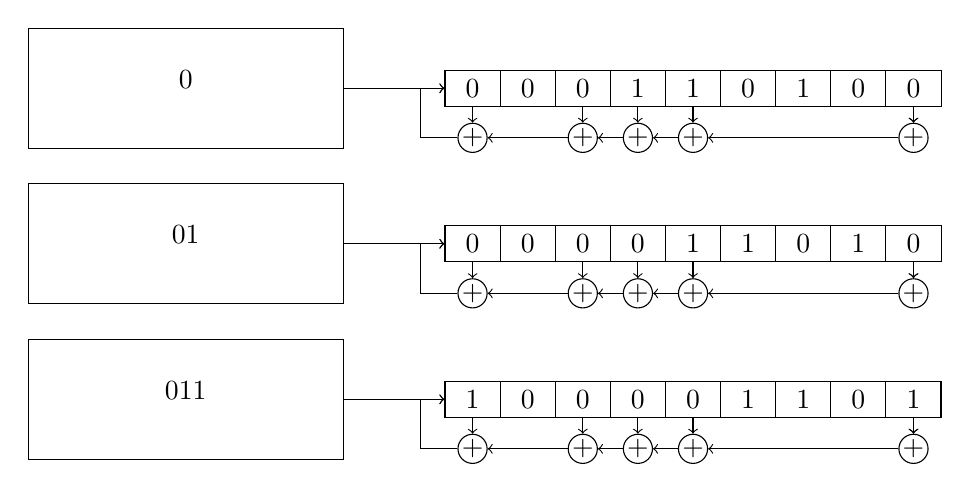
\begin{tikzpicture}
          % The LFSR chain + outputs
          \matrix (M) [matrix of math nodes,nodes={draw,minimum width=7mm},column sep=-\pgflinewidth,row sep=1.5cm]
          {
            0 & 0 & 0 & 1 & 1 & 0 & 1 & 0 & 0 \\
            0 & 0 & 0 & 0 & 1 & 1 & 0 & 1 & 0 \\
            1 & 0 & 0 & 0 & 0 & 1 & 1 & 0 & 1 \\
          };

          % taps
          \foreach \i/\j in {1/9, 1/5, 1/4, 1/3, 1/1, 2/9, 2/5, 2/4, 2/3, 2/1, 3/9, 3/5, 3/4, 3/3, 3/1}
          {\node (c-\i-\j) [circ,below=of M-\i-\j]{$+$};
            \draw[->] (M-\i-\j)--(c-\i-\j);}

          % arrows
          \draw[->] (M-1-9) edge (c-1-9) (c-1-9) edge (c-1-5) (c-1-5) edge (c-1-4) (c-1-4) edge (c-1-3) (c-1-3) edge (c-1-1) (c-1-1) -| ($(M-1-1.west)+ (-3mm,0)$)--(M-1-1);

          \draw[->] (M-2-9) edge (c-2-9) (c-2-9) edge (c-2-5) (c-2-5) edge (c-2-4) (c-2-4) edge (c-2-3) (c-2-3) edge (c-2-1) (c-2-1) -| ($(M-2-1.west)+ (-3mm,0)$)--(M-2-1);
          
          \draw[->] (M-3-9) edge (c-3-9) (c-3-9) edge (c-3-5) (c-3-5) edge (c-3-4) (c-3-4) edge (c-3-3) (c-3-3) edge (c-3-1) (c-3-1) -| ($(M-3-1.west)+ (-3mm,0)$)--(M-3-1);
          
          
          % output boxes
          \coordinate (flc1) at ($(M-1-1.south east) + (-2,1)$);
          \coordinate (frc1) at ($(M-1-1.north east) + (-6,-1)$);
          \node(s)[draw, fit=(flc1) (frc1),inner sep=0pt] {0};  
          \draw[->] (M-1-1 -| flc1)--(M-1-1);

          \coordinate (flc2) at ($(M-2-1.south east) + (-2,1)$);
          \coordinate (frc2) at ($(M-2-1.north east) + (-6,-1)$);
          \node(s)[draw, fit=(flc2) (frc2),inner sep=0pt] {01};  
          \draw[->] (M-2-1 -| flc2)--(M-2-1);

          \coordinate (flc3) at ($(M-3-1.south east) + (-2,1)$);
          \coordinate (frc3) at ($(M-3-1.north east) + (-6,-1)$);
          \node(s)[draw, fit=(flc3) (frc3),inner sep=0pt] {011};  
          \draw[->] (M-3-1 -| flc3)--(M-3-1);
          
        \end{tikzpicture}
      \end{center}
      \begin{center}
        \scalebox{1.5}{.}\\
        \scalebox{1.5}{.}\\
        \scalebox{1.5}{.}\\
      \end{center}
      \begin{center}
        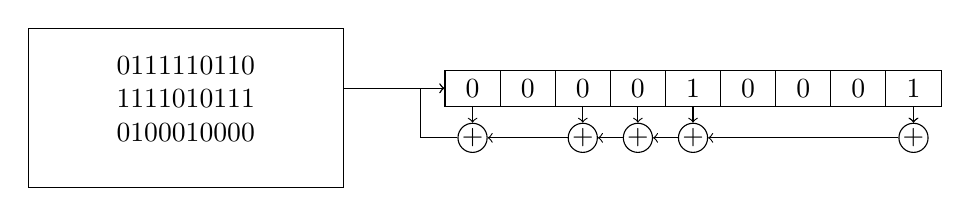
\begin{tikzpicture}
          % The LFSR chain + outputs
          \matrix (M) [matrix of math nodes,nodes={draw,minimum width=7mm},column sep=-\pgflinewidth,row sep=0.5cm]
          {
            0 & 0 & 0 & 0 & 1 & 0 & 0 & 0 & 1 \\
          };

          % taps 
          \foreach \i/\j in {1/9, 1/5, 1/4, 1/3, 1/1}
          {\node (c-\i-\j) [circ,below=of M-\i-\j]{$+$};
            \draw[->] (M-\i-\j)--(c-\i-\j);}

          % arrows
          \draw[->] (M-1-9) edge (c-1-9) (c-1-9) edge (c-1-5) (c-1-5) edge (c-1-4) (c-1-4) edge (c-1-3) (c-1-3) edge (c-1-1) (c-1-1) -| ($(M-1-1.west)+ (-3mm,0)$)--(M-1-1);
          
          % output box
          \coordinate (flc) at ($(M-1-1.south east) + (-2,1)$);
          \coordinate (frc) at ($(M-1-1.north east) + (-6,-1.5)$);
          \node(s)[draw, fit=(flc) (frc),inner sep=0pt] {
            $0111110110$\\$1111010111$\\$0100010000$
          };
          \foreach \j in {1}  
          {\draw[->] (M-\j-1 -| flc)--(M-\j-1);}
          
        \end{tikzpicture}
      \end{center}
    \end{answer}
  \item Use Vernam Cipher to encrypt the following plaintext using the bit stream generated in part b.
    P='111011000001101110110100111110'
    \begin{answer}
        $111011000001101110110100111110$ \\
        \hspace{5.8cm} $\oplus$ \\
        $011111011011110101110100010000$  \\
        --------------------------------------------- \\
        $100100011010011011000000101110$ \\
        \begin{center}
          $\bm{100100011010011011000000101110}$ 
        \end{center}
    \end{answer}
  \end{enumerate}
  
\end{enumerate}

\end{document}